\documentclass[fullscreen=true, unicode, bookmarks=false]{beamer}
\usepackage[T2A]{fontenc}
\usepackage[utf8]{inputenc}
\usepackage[english, russian]{babel}
\usepackage{amsmath}
\usepackage{amsmath,amsfonts,amssymb}
\usepackage[export]{adjustbox}
\usepackage{textgreek}
\newtheorem{rustheorem}{Теорема }
\sloppy

\setbeamertemplate{navigation symbols}{}

\usetheme{Madrid}

\usecolortheme{whale}

\usefonttheme{professionalfonts} % default family is serif

\setbeamertemplate{footline}{\hspace*{.5cm}\scriptsize{\insertshorttitle
\hspace*{50pt} \hfill\hspace*{.5cm}}\vspace{5pt}} 

\setbeamercolor{bibliography entry author}{fg=black}

\title[]{ АНАЛИЗ БИФУРКАЦИИ В НЕЛИНЕЙНОЙ КРАЕВОЙ ЗАДАЧЕ С ЗАПАЗДЫВАНИЕМ }   
\author[]{{\large Леонид Ивановский, Илья Куксёнок}} 
\date{}
\institute[]
{  }
\titlegraphic{
   \vspace{-0.5cm}
   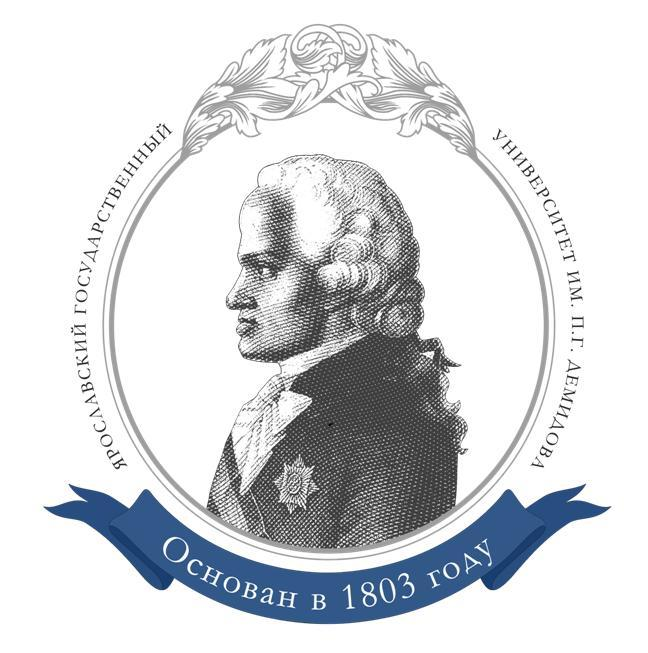
\includegraphics[scale = 0.19]{yarsu_logo.jpg}
   \hspace{0.9cm}
   
\includegraphics[scale = 0.14]{mephi_logo.png}
}

\begin{document}

\begin{frame}
\titlepage
\end{frame} 

\begin{frame}
\frametitle{ Общая формулировка задачи }
 
\begin{equation}\label{eq1}
	u' = \ddot{u} + \gamma u - u^3,
\end{equation}	

\begin{gather}\label{eq2}	
	u'(0, t) \, = 0, \\
	u'(1, t) \, = \alpha\,u(x_0, t-\tau). \nonumber
\end{gather}

$$ \alpha, \gamma \in \mathbb{R}, \quad \tau \geqslant 0, \quad x_0 \in [0, 1]. $$

\medskip
\pause

\begin{exampleblock}{}
{\large Кащенко С.А. О бифуркациях при малых возмущениях в логистическом уравнении с запаздыванием // Модел. и. анализ информ. систем, №24(2), с. 168--185 (2017). }
\end{exampleblock}

\end{frame}

\begin{frame}
\frametitle{ Нелинейная краевая задача без запаздывания}
 
\begin{equation}\label{eq3}
	u' = \ddot{u} + \gamma u - u^3,
\end{equation}	

\begin{gather}\label{eq4}	
	u'\mid_{x=0} \, = 0, \\
	u'\mid_{x=1} \, = \alpha\,u\mid_{x=x_0}. \nonumber
\end{gather}

$$ \alpha, \gamma \in \mathbb{R}, \quad x_0 \in [0, 1]. $$

\medskip

\begin{exampleblock}{}
{\large Исследование выполнено за счет гранта Российского научного фонда (проект №14-21-00158). }
\end{exampleblock}

\end{frame}

\begin{frame}
\frametitle{Нелинейная краевая задача с запаздыванием в граничном условии}
 
\begin{equation}\label{eq5}
	\dot{u}  = u'' + \gamma u - u^3,
\end{equation}	

\begin{gather}\label{eq6}	
	u'\mid_{x=0} \, = 0, \\
	u'\mid_{x=1} \, = \alpha\,u(1, t-\tau). \nonumber
\end{gather}

$$ \alpha,  \gamma \in \mathbb{R}, \quad \tau > 0. $$

\medskip

\begin{exampleblock}{}
{\large Исследование выполнено при поддержке Центра Интегрируемых Систем ЯрГУ им. П.Г. Демидова }
\end{exampleblock}

\end{frame}

\begin{frame}
\frametitle{ Упрощенная краевая задача }

$$ u(x, t) = w(x)\,\mbox{exp}\left( \lambda - \gamma t \right) $$

\bigskip
\pause
	
\begin{equation}\label{eq7}
	w'' - \lambda w = 0,
\end{equation}

\begin{gather}\label{eq8}	
	w'(0) = 0, \\
	w'(1) = \alpha\,w(x_0)e^{i \omega \tau}. \nonumber
\end{gather}

\end{frame}

\begin{frame}
\frametitle{ Граничные условия }

$$ w(x) = c \, \mbox{ch} (\mu\,x), $$

$$ \mu^2 = \lambda. $$

\vspace{1.1cm}
\pause
	
$$ x = 1: $$

\begin{gather}\label{eq9}	
	\mu \sh \mu = \alpha \ch(\mu x_0), \\
	\mu \sh \mu = \alpha \ch \mu \; e^{i \omega \tau}. \nonumber
\end{gather}

\end{frame}

\begin{frame}
\frametitle{Колебательная потеря устойчивости нулевого состояния равновесия }
	
\begin{rustheorem}
Cуществует такое $ \alpha=\alpha_{cr} $, для которого $ \mbox{Re}(\lambda_{*}) = \gamma $ и для всех остальных собственных значений задачи (7), (8) $ \mbox{Re}(\lambda) < \gamma $. 
\end{rustheorem}

\end{frame}

\begin{frame}
\frametitle{ Численное исследование } 

\begin{figure} 

\includegraphics[scale=0.25]{python.png}  
\hfill

\includegraphics[scale=0.6]{openmp.jpg} 
\end{figure}

\end{frame}

\begin{frame}
\frametitle{ Алгоритм } 

\begin{figure} 
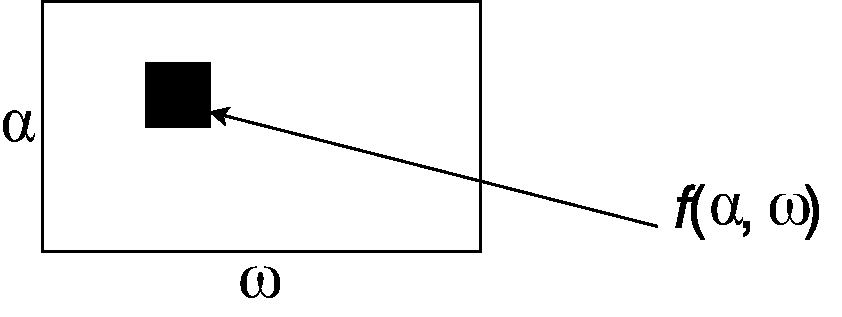
\includegraphics[scale=0.6]{Diagram.pdf}  
\end{figure}

\pause

\begin{gather}\label{eq9}	
	f(\omega, \alpha) = \mu \sh \mu - \alpha \ch(\mu x_0), \\
	f(\omega, \alpha) = \mu \sh \mu - \alpha \ch \mu \; e^{i \omega \tau}. \nonumber
\end{gather}

\pause

$$ \alpha_{cr}: \; f(\omega, \alpha_{cr}) = 0. $$

\end{frame}


\begin{frame}

\frametitle{Результаты} 

\begin{figure}
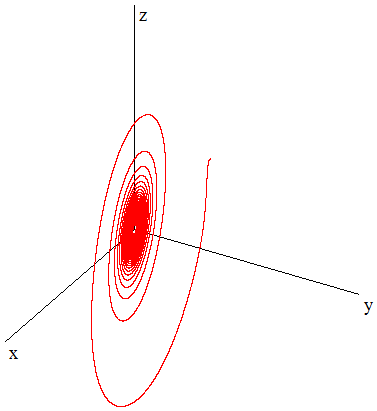
\includegraphics[scale=0.55]{AHB.png} 
\end{figure}
{\footnotesize $$ \gamma = 3.3, \quad \alpha_{cr} = -4.0, \quad x_0 = 0 $$}

\end{frame}

\begin{frame}

\frametitle{Результаты} 

\begin{figure}
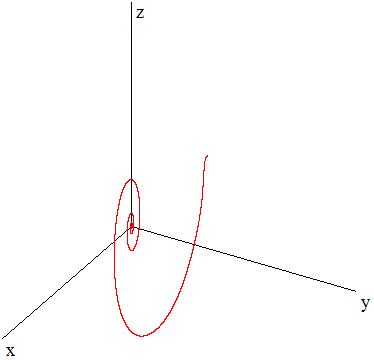
\includegraphics[scale=0.55]{AHBbefore.png} 
\end{figure}
{\footnotesize $$ \gamma = 3.3, \quad \alpha_{cr} = -2.5, \quad x_0 = 0 $$}

\end{frame}

\begin{frame}

\frametitle{Результаты} 

\begin{figure}
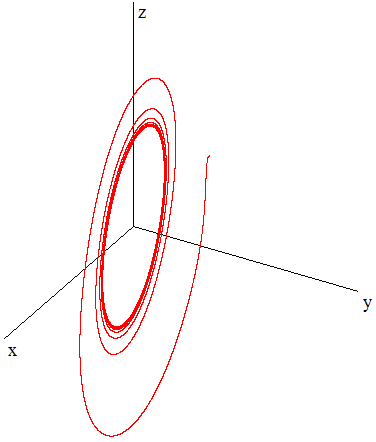
\includegraphics[scale=0.55]{AHBafter.png} 
\end{figure}
{\footnotesize $$ \gamma = 3.3, \quad \alpha_{cr} = -5.0, \quad x_0 = 0 $$}

\end{frame}

\begin{frame}
\frametitle{Нормальная форма}

\begin{equation}
	u(x,t) = \sum_{j=1}^{\infty} \varepsilon^\frac{j+1}{2}u_j (t,s,x), \quad s = \varepsilon t
\end{equation}

\vspace{1.5cm}

\begin{equation}
	u_{0}(x,t) = z(s)e^{i \omega t} w(x) + \overline{z(s)}e^{-i \omega t}\overline{w(x)}
\end{equation}

\end{frame}

\begin{frame}
\frametitle{ Система последовательно разрешимых краевых задач }

\begin{equation}
	\begin{aligned}
		\sqrt{\varepsilon}:& \quad \dot{u}_{0} = u_{0}'' + u_{0} \\
		\varepsilon:& \quad \dot{u}_{1} = u_{1}'' + u_{1} + f( u_{0}) \\
		\varepsilon^{3/2}:& \quad \dot{u}_{2} = u_{2}'' + u_{2} + g(u_{0},u_{1}) \\
	\end{aligned}
\end{equation}

\end{frame}

\begin{frame}
	\begin{equation}
		u'_{0}(0)=0
	\end{equation}

\medskip		
	
	\begin{equation}
		\begin{aligned}
			u'_{0}(1) = & \alpha_{cr}u_{0}(x_{0})\\
			u'_{0}(1) = & \alpha_{cr}u_{0}(1)e^{-i \omega \tau}\\
		\end{aligned}
	\end{equation}
	
\medskip 
	
	\begin{equation}
		u'_{2}(0)=0
	\end{equation}
	
\medskip		
	
	\begin{equation}
		\begin{aligned}
			u'_{2}(1) = & \alpha_{cr}u_{2}(x_{0}) + u_{0}(x_{0})\\
			u'_{2}(1) = & \alpha_{cr}u_{2}(1)e^{-i \omega \tau} - \alpha_{cr}\tau u_{0}(1)\\
		\end{aligned}
	\end{equation}
\end{frame}

\begin{frame}
	\begin{equation}
		u_{2}=e^{i \omega t} v(x)
	\end{equation}

\medskip		
	
	\begin{equation}
		v(x) = c_{1}(x) ch(\mu x) + c_{2}(x) sh(\mu x)
	\end{equation}

\medskip	
	
	\begin{equation}
		\begin{aligned}
			c_{1} = I_{1}(x) + q_{1} \\
			c_{2} = I_{2}(x) + q_{2} \\
		\end{aligned}
	\end{equation}
\end{frame}

\begin{frame}
\frametitle{Нормальная форма}

\begin{equation} \label{norm_form}
	\dot{z} = \phi z + d z |z|^2
\end{equation}

\vspace{1.5cm}
	
\begin{rustheorem}
	При $ Re(\phi)>0,\, Re(d)<0 \;\; \exists \varepsilon_0 > 0 \;\; \forall \varepsilon \in (0,\varepsilon_0] $
	наблюдается экспоненциально-орбитально устойчивый цикл, 
	асимптотика которого описывается формулой (14), в которой
	$z(s) = \sqrt{-\frac{Re(\phi)}{Re(d)}} \exp{\left(i \left(Im(\phi) -
	 \frac{Im(d)Re(\phi)}{Re(d)} \right) s + i\gamma \right)} $
\end{rustheorem}
\end{frame}
\begin{frame}
\frametitle{Квазианалитическое решение}
Положим 
\begin{equation}\label{kuksenok-eq2}
\mu = - \gamma + i \omega , 
\end{equation}
Тогда
\begin{equation}\label{kuksenok-eq3}
(\ref{eq7}, \ref{eq8}) \quad \rightarrow \quad
\left\{
\begin{matrix}
    \mu \sh{\mu}-\alpha \exp{(-i \omega \tau)} \ch{\mu} = 0 & \mbox{при } \tau \neq 0 \\
    \mu \sh{\mu}-\alpha  \ch{\mu} = 0 & \mbox{при } \tau = 0
\end{matrix}
\right.
\end{equation}
$$ \omega \in \mathbb{R}$$
\end{frame}
\begin{frame}
\frametitle{Квазианалитическое решение}
Получим спектр  собственных чисел
\begin{equation}\label{kuksenok-eq4}
\omega = -i(\gamma + \mu ), 
\end{equation}
Где $\mu$ может быть найдено численно из   (\ref{kuksenok-eq3})
\end{frame}
\end{document}